% !TEX root = ../main.tex

\chapter{Problemas Física Nuclear y de Partículas: Ferrer Soria}
\label{chap:problemas_ferrer_soria}

% ==============================================================================
% SECCIÓN 1: EL NÚCLEO ATÓMICO: PROPIEDADES FÍSICAS
% ==============================================================================

\section{El núcleo atómico: propiedades físicas}

\begin{problema}[Isótopos de Litio en Espectrómetro de Masas]
Los iones de litio simplemente cargados, liberados de un ánodo caliente, son acelerados mediante una diferencia de potencial de $V = 400\text{ V}$ aplicada entre el ánodo y el cátodo. Posteriormente, se les hace pasar por un orificio practicado en el cátodo y entran en una región con un campo magnético uniforme y perpendicular a la dirección del movimiento de $B = 8 \times 10^{-2}\text{ T}$, siendo los radios de sus órbitas $R_1 = 8.83\text{ cm}$ y $R_2 = 9.54\text{ cm}$, respectivamente. Calcúlense los números másicos de estos isótopos de litio.

\tcblower

\subsubsection*{1. Planteamiento físico y deducción analítica}

Un ion de litio simplemente cargado posee una carga neta positiva $q = +e$.

En primer lugar, en la región comprendida entre el ánodo y el cátodo, la energía potencial electrostática se transforma íntegramente en energía cinética:
\begin{equation}
q V = \frac{1}{2} m v^2 \implies v = \sqrt{\frac{2 q V}{m}}
\end{equation}

En segundo lugar, al ingresar en la región de campo magnético uniforme $\vec{B}$ perpendicular a la velocidad ($\vec{v} \perp \vec{B}$), la fuerza magnética de Lorentz actúa como fuerza centrípeta, obligando al ion a describir una trayectoria circular de radio $R$:
\begin{equation}
F_m = q v B = \frac{m v^2}{R} \implies m = \frac{q B R}{v}
\end{equation}

Sustituyendo la expresión de la velocidad $v$ en la ecuación de la masa y elevando al cuadrado ambos miembros:
\begin{equation}
m = \frac{q B R}{\sqrt{\frac{2 q V}{m}}} \implies m^2 = \frac{q^2 B^2 R^2 m}{2 q V} \implies m = \frac{q B^2 R^2}{2 V}
\end{equation}

\subsubsection*{2. Identificación de isótopos mediante la relación de radios}

Dado que la carga $q$, el potencial $V$ y el campo magnético $B$ son idénticos para ambos isótopos, la masa de cada ion es directamente proporcional al cuadrado de su radio orbital ($m \propto R^2$). El cociente de masas viene dado por:
\begin{equation}
\frac{m_2}{m_1} = \left( \frac{R_2}{R_1} \right)^2 = \left( \frac{9.54\text{ cm}}{8.83\text{ cm}} \right)^2 = (1.0804)^2 \approx 1.1673
\end{equation}

Si comparamos este valor con la razón entre los enteros $7$ y $6$:
\begin{equation}
\frac{7}{6} \approx 1.1667
\end{equation}

La concordancia confirma que los números másicos de los isótopos de litio son $A_1 = 6$ y $A_2 = 7$.

\subsubsection*{3. Cálculo explícito de las masas atómicas}

Utilizando las constantes fundamentales en el Sistema Internacional:
\begin{itemize}
    \item Carga elemental: $e = 1.602 \times 10^{-19}\text{ C}$
    \item Unidad de masa atómica: $1\text{ u} = 1.6605 \times 10^{-27}\text{ kg}$
    \item Potencial de aceleración: $V = 400\text{ V}$
    \item Campo magnético: $B = 8 \times 10^{-2}\text{ T}$
\end{itemize}

\paragraph{Isótopo 1 ($R_1 = 0.0883\text{ m}$):}
\begin{equation}
m_1 = \frac{(1.602 \times 10^{-19}\text{ C}) \times (8 \times 10^{-2}\text{ T})^2 \times (0.0883\text{ m})^2}{2 \times 400\text{ V}} = 9.990 \times 10^{-27}\text{ kg}
\end{equation}
Expresando la masa en unidades $u$:
\begin{equation}
m_1 = \frac{9.990 \times 10^{-27}\text{ kg}}{1.6605 \times 10^{-27}\text{ kg/u}} \approx 6.016\text{ u} \implies A_1 = 6 \quad ({}^{6}\text{Li})
\end{equation}

\paragraph{Isótopo 2 ($R_2 = 0.0954\text{ m}$):}
\begin{equation}
m_2 = \frac{(1.602 \times 10^{-19}\text{ C}) \times (8 \times 10^{-2}\text{ T})^2 \times (0.0954\text{ m})^2}{2 \times 400\text{ V}} = 1.166 \times 10^{-26}\text{ kg}
\end{equation}
Expresando la masa en unidades $u$:
\begin{equation}
m_2 = \frac{1.166 \times 10^{-26}\text{ kg}}{1.6605 \times 10^{-27}\text{ kg/u}} \approx 7.022\text{ u} \implies A_2 = 7 \quad ({}^{7}\text{Li})
\end{equation}

\subsubsection*{4. Esquema del Experimento}

\begin{center}
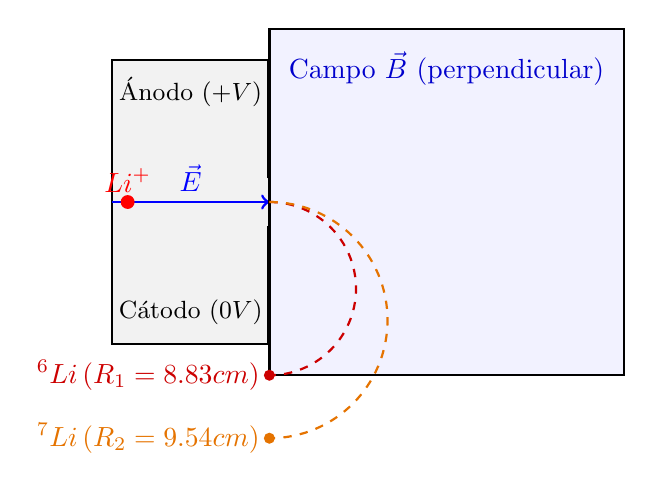
\begin{tikzpicture}[scale=1.0]
  % Región del Campo Eléctrico
  \draw[thick, fill=gray!10] (0,-1.8) rectangle (2,1.8);
  \node at (1, 1.4) {\small Ánodo ($+V$)};
  \node at (1, -1.4) {\small Cátodo ($0\text{ V}$)};
  \draw[->, line width=1pt, blue] (0,0) -- (2,0) node[midway, above] {$\vec{E}$};
  \fill[red] (0.2,0) circle (2.5pt) node[above] {$\text{Li}^+$};
  
  % Cátodo con orificio
  \draw[line width=2pt] (2,-1.8) -- (2,-0.3);
  \draw[line width=2pt] (2,0.3) -- (2,1.8);
  
  % Región del Campo Magnético
  \draw[thick, fill=blue!5] (2,-2.2) rectangle (6.5,2.2);
  \node[blue!80!black] at (4.25, 1.7) {Campo $\vec{B}$ (perpendicular)};
  
  % Trayectorias semicirculares
  \draw[thick, dashed, red!80!black] (2,0) arc (90:-90:1.1);
  \draw[thick, dashed, orange!90!black] (2,0) arc (90:-90:1.5);
  
  % Radios e Isótopos
  \fill[red!80!black] (2,-2.2) circle (2pt) node[left] {${}^6\text{Li}\,(R_1 = 8.83\text{ cm})$};
  \fill[orange!90!black] (2,-3.0) circle (2pt) node[left] {${}^7\text{Li}\,(R_2 = 9.54\text{ cm})$};
\end{tikzpicture}
\end{center}

\end{problema}
\newpage
\begin{problema}[Diferencia de Energía de Ligadura y Radio Nuclear de Isóbaros Espejo (${}^{15}\text{O}$ y ${}^{15}\text{N}$)]
    \begin{enumerate}[label=\alph*)]
        \item Utilizando como datos las masas atómicas del ${}^{15}\text{O}$ y del ${}^{15}\text{N}$, calcular la diferencia entre sus energías de ligadura.
        \item Suponiendo que dicha diferencia se debe exclusivamente a la diferencia entre sus energías culombianas, encontrar el valor del radio nuclear común $R$ para el ${}^{15}\text{O}$ y el ${}^{15}\text{N}$.
    \end{enumerate}
\textbf{Datos:} $M({}^{15}\text{O}) = 15.003065\text{ u}$, $M({}^{15}\text{N}) = 15.000109\text{ u}$, $M({}^1\text{H}) = 1.007825\text{ u}$, $m_n = 1.008665\text{ u}$, $1\text{ u} \cdot c^2 = 931.5\text{ MeV}$, $e^2/(4\pi\varepsilon_0) = 1.440\text{ MeV}\cdot\text{fm}$.

\tcblower

\subsubsection*{a) Diferencia entre las energías de ligadura}

La energía de ligadura de un núclido ${}_Z^A Y$ compuesto por $Z$ protones y $N = A - Z$ neutrones se define como:
\begin{equation}
B(Z,A) = \left[ Z \, M({}^1\text{H}) + (A - Z) \, m_n - M(Z,A) \right] c^2
\end{equation}

Escribimos las expresiones correspondientes para los dos isóbaros espejo de $A = 15$:
\begin{itemize}
    \item \textbf{Oxígeno-15 ($Z = 8, N = 7$):}
    \begin{equation}
    B({}^{15}\text{O}) = \left[ 8 \, M({}^1\text{H}) + 7 \, m_n - M({}^{15}\text{O}) \right] c^2
    \end{equation}
    \item \textbf{Nitrógeno-15 ($Z = 7, N = 8$):}
    \begin{equation}
    B({}^{15}\text{N}) = \left[ 7 \, M({}^1\text{H}) + 8 \, m_n - M({}^{15}\text{N}) \right] c^2
    \end{equation}
\end{itemize}

Restando la energía de ligadura del ${}^{15}\text{N}$ de la del ${}^{15}\text{O}$:
\begin{equation}
\Delta B \equiv B({}^{15}\text{O}) - B({}^{15}\text{N}) = \left[ M({}^1\text{H}) - m_n - M({}^{15}\text{O}) + M({}^{15}\text{N}) \right] c^2
\end{equation}

Sustituyendo los valores numéricos de las masas:
\begin{align}
\Delta m &= (1.007825\text{ u} - 1.008665\text{ u}) - (15.003065\text{ u} - 15.000109\text{ u}) \nonumber \\
&= -0.000840\text{ u} - 0.002956\text{ u} = -0.003796\text{ u}
\end{align}

Convertimos el defecto de masa a unidades de energía:
\begin{equation}
\Delta B = (-0.003796\text{ u}) \times 931.5\text{ MeV/u} \approx -3.536\text{ MeV}
\end{equation}

Por lo tanto, la energía de ligadura del ${}^{15}\text{N}$ supera a la del ${}^{15}\text{O}$ en $3.536\text{ MeV}$:
\begin{equation}
B({}^{15}\text{N}) - B({}^{15}\text{O}) = 3.536\text{ MeV}
\end{equation}

\newpage

\subsubsection*{b) Cálculo del radio nuclear a partir de la energía de Coulomb}

Dado que los núcleos ${}^{15}\text{O}$ y ${}^{15}\text{N}$ forman un par de \textit{isóbaros espejo} ($Z_1 = 8, N_1 = 7$ frente a $Z_2 = 7, N_2 = 8$), la interacción fuerte entre nucleones es simétrica de carga ($V_{pp} \approx V_{nn}$). La diferencia en su energía de ligadura se debe fundamentalmente a la mayor repulsión electrostática presente en el ${}^{15}\text{O}$ ($Z = 8$).

Modelando ambos núcleos como esferas homogéneamente cargadas de radio equivalente $R$, la energía culombiana viene dada por la expresión que contabiliza el número de pares de protones $Z(Z-1)/2$:
\begin{equation}
E_C = \frac{3}{5} \frac{1}{4\pi\varepsilon_0} \frac{Z(Z-1) e^2}{R}
\end{equation}

Puesto que la energía de ligadura se reduce con la repulsión electrostática ($B = B_{\text{fuerte}} - E_C$), la diferencia de energías de ligadura satisface:
\begin{equation}
B({}^{15}\text{N}) - B({}^{15}\text{O}) = E_C({}^{15}\text{O}) - E_C({}^{15}\text{N}) = \Delta E_C = 3.536\text{ MeV}
\end{equation}

Evaluamos la diferencia de energía culombiana:
\begin{equation}
\Delta E_C = \frac{3}{5} \frac{e^2}{4\pi\varepsilon_0 R} \left[ Z_1(Z_1 - 1) - Z_2(Z_2 - 1) \right]
\end{equation}

Para $Z_1 = 8$ y $Z_2 = 7$:
\begin{equation}
Z_1(Z_1 - 1) - Z_2(Z_2 - 1) = 8 \times 7 - 7 \times 6 = 56 - 42 = 14
\end{equation}

Sustituyendo las constantes:
\begin{equation}
\Delta E_C = \frac{3}{5} \frac{1.440\text{ MeV}\cdot\text{fm}}{R} \times 14 = \frac{12.096\text{ MeV}\cdot\text{fm}}{R}
\end{equation}

Igualando a $\Delta E_C = 3.536\text{ MeV}$ y despejando el radio nuclear $R$:
\begin{equation}
R = \frac{12.096\text{ MeV}\cdot\text{fm}}{3.536\text{ MeV}} \approx 3.42\text{ fm}
\end{equation}

\textit{Nota metodológica:} Si en lugar de $Z(Z-1)$ se adopta la aproximación simplificada $E_C \propto Z^2$, el factor vale $8^2 - 7^2 = 15$, resultando $R = \frac{12.96}{3.536} \approx 3.67\text{ fm}$. El valor $R \approx 3.42\text{ fm}$ resulta más preciso y concuerda perfectamente con la constante de radio nuclear $r_0 \approx 1.38\text{ fm}$ para $R = r_0 A^{1/3} = 1.38 \times 15^{1/3} \approx 3.41\text{ fm}$.

\subsubsection*{Esquema del Par de Núcleos Espejo}

\begin{center}
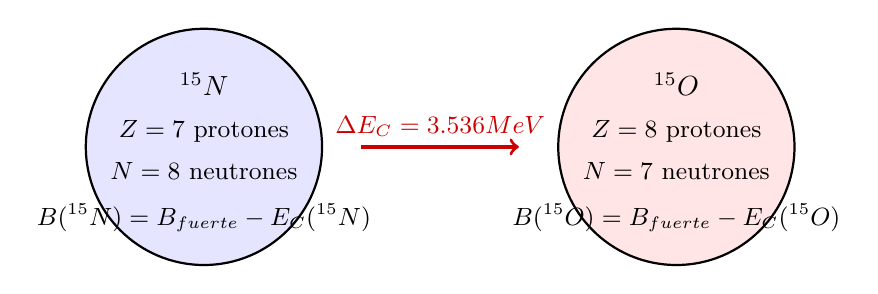
\begin{tikzpicture}[scale=1.0]
  % Núcleo 15N
  \draw[thick, fill=blue!10] (0,0) circle (1.5);
  \node at (0, 0.8) {\textbf{${}^{15}\text{N}$}};
  \node at (0, 0.2) {\small $Z = 7$ protones};
  \node at (0, -0.3) {\small $N = 8$ neutrones};
  \node at (0, -0.9) {\small $B({}^{15}\text{N}) = B_{\text{fuerte}} - E_C({}^{15}\text{N})$};

  % Flecha de comparación
  \draw[->, line width=1.2pt, red!80!black] (2.0,0) -- (4.0,0) node[midway, above] {\small $\Delta E_C = 3.536\text{ MeV}$};

  % Núcleo 15O
  \draw[thick, fill=red!10] (6.0,0) circle (1.5);
  \node at (6.0, 0.8) {\textbf{${}^{15}\text{O}$}};
  \node at (6.0, 0.2) {\small $Z = 8$ protones};
  \node at (6.0, -0.3) {\small $N = 7$ neutrones};
  \node at (6.0, -0.9) {\small $B({}^{15}\text{O}) = B_{\text{fuerte}} - E_C({}^{15}\text{O})$};
\end{tikzpicture}
\end{center}

\end{problema}
\newpage
\begin{problema}[Relación de Energías Culombianas entre Distribuciones Volumétrica y Superficial]
Supóngase que la carga eléctrica $Q = Z e$ de un cierto núcleo:
\begin{enumerate}[label=\alph*)]
    \item Se distribuye homogéneamente en todo el volumen de una esfera de radio $R$.
    \item Se distribuye homogéneamente sólo sobre la superficie de dicha esfera.
\end{enumerate}
Calcular el valor de la relación $U_c(\text{vol}) / U_c(\text{sup})$ entre las correspondientes energías potenciales electrostáticas de Coulomb.

\tcblower

\subsubsection*{1. Expresión general de la energía electrostática}

La energía potencial electrostática (o energía de Coulomb) $U_c$ de una distribución continua de carga representa el trabajo necesario para ensamblar dicha distribución frente a la repulsión electrostática:
\begin{equation}
U_c = \frac{1}{2} \int V(\vec{r}) \, dq
\end{equation}
donde $V(\vec{r})$ es el potencial electrostático generado por toda la distribución en la posición del elemento diferencial de carga $dq$.

\subsubsection*{a) Distribución volumétrica homogénea}

Para una carga total $Q = Z e$ repartida uniformemente en una esfera sólida de radio $R$, la densidad volumétrica constante de carga es:
\begin{equation}
\rho = \frac{Q}{V_{\text{esfera}}} = \frac{Q}{\frac{4}{3}\pi R^3}
\end{equation}

El potencial electrostático $V(r)$ en un punto interior de la esfera ($r \le R$) se calcula mediante la ley de Gauss integrando el campo eléctrico interior $E(r) = \frac{Q r}{4\pi\varepsilon_0 R^3}$:
\begin{equation}
V(r) = V(R) - \int_R^r E(r') \, dr' = \frac{Q}{4\pi\varepsilon_0 R} + \frac{Q}{8\pi\varepsilon_0 R^3} (R^2 - r^2) = \frac{Q}{4\pi\varepsilon_0 \cdot 2R^3} \left( 3R^2 - r^2 \right)
\end{equation}

Sustituyendo $dq = \rho \, d^3r = \rho \cdot 4\pi r^2 dr$ en la integral de energía:
\begin{equation}
U_c(\text{vol}) = \frac{1}{2} \int_0^R V(r) \, \rho \cdot 4\pi r^2 dr
\end{equation}

Sustituyendo las expresiones de $\rho$ y $V(r)$:
\begin{align}
U_c(\text{vol}) &= \frac{1}{2} \left( \frac{Q}{\frac{4}{3}\pi R^3} \right) \left( \frac{Q}{8\pi\varepsilon_0 R^3} \right) 4\pi \int_0^R (3R^2 r^2 - r^4) \, dr \nonumber \\
&= \frac{3 Q^2}{16\pi\varepsilon_0 R^6} \left[ 3R^2 \frac{R^3}{3} - \frac{R^5}{5} \right] = \frac{3 Q^2}{16\pi\varepsilon_0 R^6} \left( \frac{4 R^5}{5} \right)
\end{align}

Obteniéndose el valor clásico para la esfera homogénea:
\begin{equation}
U_c(\text{vol}) = \frac{3}{5} \frac{Q^2}{4\pi\varepsilon_0 R} = \frac{3}{5} \frac{Z^2 e^2}{4\pi\varepsilon_0 R}
\end{equation}

\subsubsection*{b) Distribución superficial homogénea}

Para una carga $Q = Z e$ distribuida uniformemente sobre la corteza esférica de radio $R$, la densidad de carga es:
\begin{equation}
\sigma = \frac{Q}{S_{\text{esfera}}} = \frac{Q}{4\pi R^2}
\end{equation}

En todos los puntos de la superficie esférica ($r = R$), el potencial electrostático es constante e igual a:
\begin{equation}
V(R) = \frac{Q}{4\pi\varepsilon_0 R}
\end{equation}

Sustituyendo $dq = \sigma \, d^2r$ en la integral de energía:
\begin{equation}
U_c(\text{sup}) = \frac{1}{2} \int_S V(R) \, \sigma \, d^2r = \frac{1}{2} V(R) \int_S \sigma \, d^2r = \frac{1}{2} V(R) \cdot Q
\end{equation}

Sustituyendo la expresión del potencial $V(R)$:
\begin{equation}
U_c(\text{sup}) = \frac{1}{2} \left( \frac{Q}{4\pi\varepsilon_0 R} \right) Q = \frac{1}{2} \frac{Q^2}{4\pi\varepsilon_0 R} = \frac{Q^2}{8\pi\varepsilon_0 R}
\end{equation}

\subsubsection*{c) Relación de energías de Coulomb}

Calculamos la razón entre ambas energías potenciales electrostáticas:
\begin{equation}
\frac{U_c(\text{vol})}{U_c(\text{sup})} = \frac{\frac{3}{5} \frac{Q^2}{4\pi\varepsilon_0 R}}{\frac{1}{2} \frac{Q^2}{4\pi\varepsilon_0 R}} = \frac{3/5}{1/2} = \frac{6}{5} = 1.2
\end{equation}

\textbf{Conclusión:} La energía de repulsión culombiana de un núcleo modelado como una esfera cargada homogénea es un $20\%$ superior ($\times 1.2$) a la de una corteza esférica del mismo radio, debido al trabajo necesario para empaquetar la carga dentro del volumen interior.

\subsubsection*{Esquema de las Distribuciones de Carga}

\begin{center}
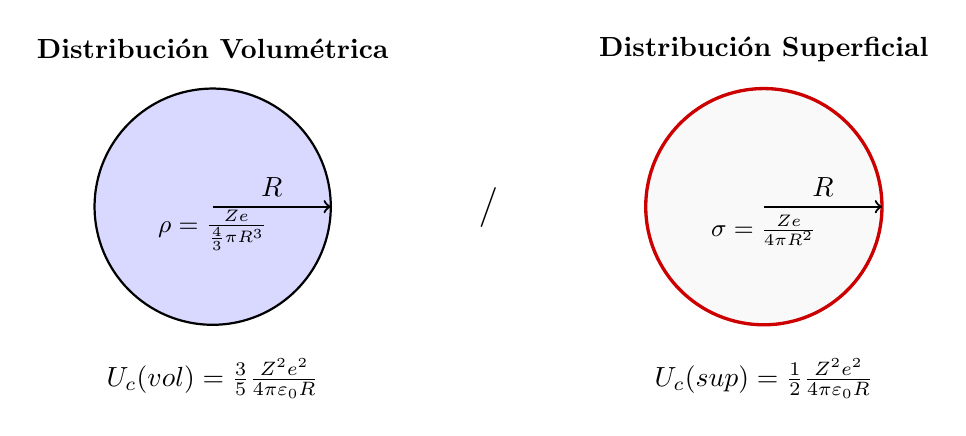
\begin{tikzpicture}[scale=1.0]
  % Esfera Volumétrica
  \draw[thick, fill=blue!15] (-3.5,0) circle (1.5);
  \node at (-3.5, 2) {\textbf{Distribución Volumétrica}};
  \node at (-3.5, -0.3) {\small $\rho = \frac{Ze}{\frac{4}{3}\pi R^3}$};
  \draw[->, thick] (-3.5,0) -- (-2.0,0) node[midway, above] {$R$};
  \node[below] at (-3.5, -1.8) {$U_c(\text{vol}) = \frac{3}{5} \frac{Z^2 e^2}{4\pi\varepsilon_0 R}$};

  % Simbolo de división
  \node at (0,0) {\Large $\mathbf{\Big/}$};

  % Esfera Superficial
  \draw[very thick, fill=gray!5, draw=red!80!black] (3.5,0) circle (1.5);
  \node at (3.5, 2) {\textbf{Distribución Superficial}};
  \node at (3.5, -0.3) {\small $\sigma = \frac{Ze}{4\pi R^2}$};
  \draw[->, thick] (3.5,0) -- (5.0,0) node[midway, above] {$R$};
  \node[below] at (3.5, -1.8) {$U_c(\text{sup}) = \frac{1}{2} \frac{Z^2 e^2}{4\pi\varepsilon_0 R}$};
\end{tikzpicture}
\end{center}

\end{problema}

\newpage
\begin{problema}[Factor de Forma Dipolar del Protón y Radio Cuadrático Medio]
Demostrar que a partir de una distribución de carga exponencial para el protón, de la forma:
\begin{equation}
\rho(r) = \rho_0 \exp(-M_v r)
\end{equation}
el factor de forma que se obtiene corresponde a la denominada fórmula del dipolo:
\begin{equation}
G(q^2) = \left[ 1 + \frac{q^2}{M_v^2} \right]^{-2}
\end{equation}
Comprobar que para $M_v = 0.84\text{ GeV}$ el radio cuadrático medio vale aproximadamente $0.8\text{ fm}$.

\tcblower

\subsubsection*{1. Normalización de la densidad de carga}

Consideramos una distribución esféricamente simétrica de carga para el protón normalizada a la unidad, de modo que $\int \rho(\vec{r}) \, d^3r = 1$. Integrando en coordenadas esféricas:
\begin{equation}
\int_0^\infty 4\pi r^2 \rho_0 e^{-M_v r} dr = 1
\end{equation}

Utilizando la propiedad de la función Gamma $\int_0^\infty r^n e^{-a r} dr = \frac{n!}{a^{n+1}}$ para $n=2$ y $a=M_v$:
\begin{equation}
4\pi \rho_0 \frac{2!}{M_v^3} = \frac{8\pi \rho_0}{M_v^3} = 1 \implies \rho_0 = \frac{M_v^3}{8\pi}
\end{equation}

\subsubsection*{2. Obtención del Factor de Forma $G(q^2)$}

El factor de forma electromagnético $G(q^2)$ se define como la transformada de Fourier tridimensional de la densidad espacial de carga $\rho(\vec{r})$ para una transferencia de momento $\vec{q}$:
\begin{equation}
G(q^2) = \int e^{i \vec{q} \cdot \vec{r}} \rho(\vec{r}) \, d^3r
\end{equation}

Para una distribución esféricamente simétrica $\rho(r)$, tras realizar la integración sobre las variables angulares se obtiene:
\begin{equation}
G(q^2) = \frac{4\pi}{q} \int_0^\infty r \sin(qr) \rho(r) \, dr
\end{equation}
donde $q = |\vec{q}|/\hbar$ representa el módulo de la transferencia de momento.

Sustituyendo la densidad exponencial $\rho(r) = \rho_0 e^{-M_v r}$:
\begin{equation}
G(q^2) = \frac{4\pi \rho_0}{q} \int_0^\infty r \sin(qr) e^{-M_v r} \, dr
\end{equation}

La integral analítica de la forma $\int_0^\infty r e^{-a r} \sin(b r) \, dr = \frac{2 a b}{(a^2 + b^2)^2}$ proporciona:
\begin{equation}
\int_0^\infty r \sin(qr) e^{-M_v r} \, dr = \frac{2 M_v q}{(M_v^2 + q^2)^2}
\end{equation}

Sustituyendo este resultado en la expresión del factor de forma:
\begin{equation}
G(q^2) = \frac{4\pi \rho_0}{q} \frac{2 M_v q}{(M_v^2 + q^2)^2} = \frac{8\pi \rho_0 M_v}{(M_v^2 + q^2)^2}
\end{equation}

Reemplazando la constante de normalización $\rho_0 = \frac{M_v^3}{8\pi}$:
\begin{equation}
G(q^2) = \frac{8\pi \left(\frac{M_v^3}{8\pi}\right) M_v}{(M_v^2 + q^2)^2} = \frac{M_v^4}{(M_v^2 + q^2)^2} = \left[ 1 + \frac{q^2}{M_v^2} \right]^{-2}
\end{equation}

queda demostrada la fórmula del dipolo.

\subsubsection*{3. Cálculo del radio cuadrático medio $\langle r^2 \rangle$}

El radio cuadrático medio de carga se puede calcular de dos formas equivalentes:

\paragraph{Método A: A partir de la distribución de carga}
\begin{equation}
\langle r^2 \rangle = \int r^2 \rho(\vec{r}) \, d^3r = 4\pi \rho_0 \int_0^\infty r^4 e^{-M_v r} \, dr = 4\pi \left(\frac{M_v^3}{8\pi}\right) \frac{4!}{M_v^5} = \frac{12}{M_v^2}
\end{equation}

\paragraph{Método B: A partir del desarrollo del factor de forma}
A bajas transferencias de momento ($q^2 \to 0$), el factor de forma admite el desarrollo en serie:
\begin{equation}
G(q^2) = 1 - \frac{1}{6} \langle r^2 \rangle q^2 + \mathcal{O}(q^4)
\end{equation}

Desarrollando la fórmula dipolar por el binomio de Newton para $q^2 \ll M_v^2$:
\begin{equation}
G(q^2) = \left( 1 + \frac{q^2}{M_v^2} \right)^{-2} = 1 - 2 \frac{q^2}{M_v^2} + \mathcal{O}(q^4)
\end{equation}

Igualando los términos de primer orden en $q^2$:
\begin{equation}
\frac{1}{6} \langle r^2 \rangle = \frac{2}{M_v^2} \implies \langle r^2 \rangle = \frac{12}{M_v^2}
\end{equation}

Por consiguiente, la raíz del radio cuadrático medio ($r_{\text{rms}}$) es:
\begin{equation}
r_{\text{rms}} \equiv \sqrt{\langle r^2 \rangle} = \frac{\sqrt{12}}{M_v} = \frac{2\sqrt{3}}{M_v}
\end{equation}

\subsubsection*{4. Comprobación numérica}

Dado el valor de la masa efectiva $M_v = 0.84\text{ GeV}$, utilizamos la constante de conversión en unidades naturales ($\hbar c = 0.1973\text{ GeV}\cdot\text{fm}$):
\begin{equation}
M_v = \frac{0.84\text{ GeV}}{0.1973\text{ GeV}\cdot\text{fm}} \approx 4.257\text{ fm}^{-1}
\end{equation}

Sustituyendo en la expresión de $r_{\text{rms}}$:
\begin{equation}
r_{\text{rms}} = \frac{2\sqrt{3}}{4.257\text{ fm}^{-1}} \approx \frac{3.464}{4.257}\text{ fm} \approx 0.814\text{ fm} \approx 0.8\text{ fm}
\end{equation}

Se comprueba así que una densidad de carga exponencial con masa $M_v = 0.84\text{ GeV}$ describe adecuadamente la dimensión espacial del protón con un radio rms de $0.8\text{ fm}$.

\subsubsection*{5. Esquema Representativo}

\begin{center}
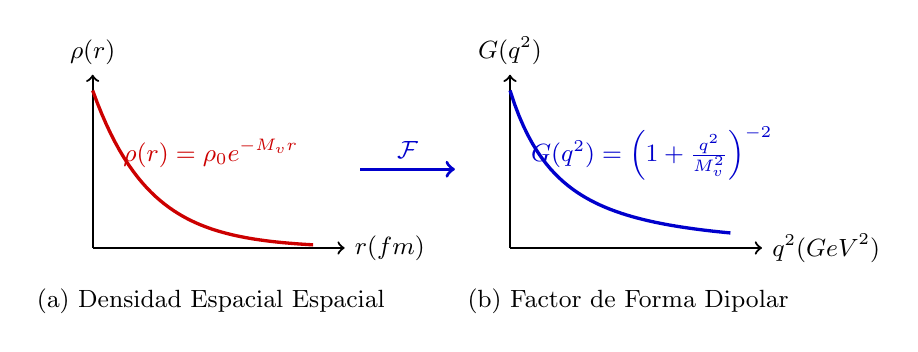
\begin{tikzpicture}[scale=1.0]
  % Gráfica Densidad Exponencial
  \begin{scope}[shift={(-3.5,0)}]
    \draw[->, thick] (0,0) -- (3.2,0) node[right] {\small $r\text{ (fm)}$};
    \draw[->, thick] (0,0) -- (0,2.2) node[above] {\small $\rho(r)$};
    \draw[red!80!black, very thick, domain=0:2.8, samples=50] plot (\x, {2.0*exp(-1.4*\x)});
    \node[red!80!black] at (1.5,1.2) {\small $\rho(r) = \rho_0 e^{-M_v r}$};
    \node[below] at (1.5,-0.4) {\small (a) Densidad Espacial Espacial};
  \end{scope}

  % Flecha Transformada de Fourier
  \draw[->, line width=1.2pt, blue!80!black] (-0.1,1.0) -- (1.1,1.0) node[midway, above] {\small $\mathcal{F}$};

  % Gráfica Factor de Forma Dipolar
  \begin{scope}[shift={(1.8,0)}]
    \draw[->, thick] (0,0) -- (3.2,0) node[right] {\small $q^2\text{ (GeV}^2\text{)}$};
    \draw[->, thick] (0,0) -- (0,2.2) node[above] {\small $G(q^2)$};
    \draw[blue!80!black, very thick, domain=0:2.8, samples=50] plot (\x, {2.0/(1.0 + 0.8*\x)^2});
    \node[blue!80!black] at (1.8,1.2) {\small $G(q^2) = \left(1 + \frac{q^2}{M_v^2}\right)^{-2}$};
    \node[below] at (1.5,-0.4) {\small (b) Factor de Forma Dipolar};
  \end{scope}
\end{tikzpicture}
\end{center}

\end{problema}

\newpage

\begin{problema}[Energía Máxima del Electrón en la Desintegración $\beta^-$ del ${}^{31}\text{Si}$]
A partir de las masas atómicas del hidrógeno ($1.0078\text{ u}$), del deuterio ($2.0141\text{ u}$) y del helio ($4.0025\text{ u}$), y conociendo los valores $Q$ de las siguientes reacciones nucleares:
\begin{align}
{}^{31}\text{P}(d,\alpha){}^{29}\text{Si}: & \quad Q_1 = 8.158\text{ MeV} \\
{}^{29}\text{Si}(d,p){}^{30}\text{Si}: & \quad Q_2 = 8.388\text{ MeV} \\
{}^{30}\text{Si}(d,p){}^{31}\text{Si}: & \quad Q_3 = 4.364\text{ MeV}
\end{align}
Calcular la energía cinética máxima del electrón emitido en la desintegración $\beta^-$ del ${}^{31}\text{Si}$.

\tcblower

\subsubsection*{1. Planteamiento de las reacciones y balance energético}

Escribimos explícitamente las tres reacciones nucleares con sus respectivos balances de energía ($Q_i$):
\begin{enumerate}[label=\arabic*)]
    \item ${}^{31}\text{P} + d \longrightarrow {}^{29}\text{Si} + \alpha + Q_1$
    \begin{equation}
    Q_1 = \left[ M({}^{31}\text{P}) + M(d) - M({}^{29}\text{Si}) - M(\alpha) \right] c^2 = 8.158\text{ MeV}
    \end{equation}

    \item ${}^{29}\text{Si} + d \longrightarrow {}^{30}\text{Si} + p + Q_2$
    \begin{equation}
    Q_2 = \left[ M({}^{29}\text{Si}) + M(d) - M({}^{30}\text{Si}) - M(p) \right] c^2 = 8.388\text{ MeV}
    \end{equation}

    \item ${}^{30}\text{Si} + d \longrightarrow {}^{31}\text{Si} + p + Q_3$
    \begin{equation}
    Q_3 = \left[ M({}^{30}\text{Si}) + M(d) - M({}^{31}\text{Si}) - M(p) \right] c^2 = 4.364\text{ MeV}
    \end{equation}
\end{enumerate}

donde $p \equiv {}^1\text{H}$, $d \equiv {}^2\text{H}$ y $\alpha \equiv {}^4\text{He}$.

\subsubsection*{2. Combinación de reacciones (Suma del ciclo nuclear)}

Sumando miembro a miembro las tres reacciones nucleares, los isótopos intermedios ${}^{29}\text{Si}$ y ${}^{30}\text{Si}$ se cancelan algebraicamente:
\begin{equation}
{}^{31}\text{P} + 3d \longrightarrow {}^{31}\text{Si} + \alpha + 2p + (Q_1 + Q_2 + Q_3)
\end{equation}

Sumando las expresiones analíticas de $Q_1$, $Q_2$ y $Q_3$:
\begin{equation}
Q_1 + Q_2 + Q_3 = \left[ M({}^{31}\text{P}) + 3 M(d) - M({}^{31}\text{Si}) - M(\alpha) - 2 M(p) \right] c^2
\end{equation}

Despejando la diferencia de masas entre el ${}^{31}\text{Si}$ y el ${}^{31}\text{P}$:
\begin{equation}
\left[ M({}^{31}\text{Si}) - M({}^{31}\text{P}) \right] c^2 = \left[ 3 M(d) - M(\alpha) - 2 M(p) \right] c^2 - (Q_1 + Q_2 + Q_3)
\end{equation}

\subsubsection*{3. Cinemática de la desintegración $\beta^-$ del ${}^{31}\text{Si}$}

El núcleo de ${}^{31}\text{Si}$ se desintegra mediante emisión $\beta^-$ hacia el estado fundamental del ${}^{31}\text{P}$:
\begin{equation}
{}^{31}\text{Si} \longrightarrow {}^{31}\text{P} + e^- + \bar{\nu}_e
\end{equation}

El valor $Q_{\beta^-}$ de la desintegración expresado en términos de masas atómicas neutras (donde la masa de los electrones orbitales queda contabilizada automáticamente) es:
\begin{equation}
Q_{\beta^-} = \left[ M({}^{31}\text{Si}) - M({}^{31}\text{P}) \right] c^2
\end{equation}

Puesto que el neutrino transporta una fracción variable de energía de forma continua, la energía cinética del electrón alcanza su valor máximo $T_{e,\text{máx}}$ cuando la energía cinética del antineutrino es prácticamente nula ($T_{\bar{\nu}} \to 0$):
\begin{equation}
T_{e,\text{máx}} \approx Q_{\beta^-} = \left[ M({}^{31}\text{Si}) - M({}^{31}\text{P}) \right] c^2
\end{equation}

\subsubsection*{4. Cálculo numérico}

\paragraph{a) Suma de las energías de reacción:}
\begin{equation}
Q_1 + Q_2 + Q_3 = 8.158\text{ MeV} + 8.388\text{ MeV} + 4.364\text{ MeV} = 20.910\text{ MeV}
\end{equation}

\paragraph{b) Balance de masa de las partículas ligeras:}
\begin{align}
\Delta m_{\text{ligero}} &= 3 M(d) - M(\alpha) - 2 M(p) \nonumber \\
&= 3(2.0141\text{ u}) - 4.0025\text{ u} - 2(1.0078\text{ u}) \nonumber \\
&= 6.0423\text{ u} - 4.0025\text{ u} - 2.0156\text{ u} = 0.0242\text{ u}
\end{align}

Convertimos el defecto de masa ligero a energía ($1\text{ u} \cdot c^2 = 931.5\text{ MeV}$):
\begin{equation}
E_{\text{ligero}} = 0.0242\text{ u} \times 931.5\text{ MeV/u} \approx 22.542\text{ MeV}
\end{equation}

\paragraph{c) Energía cinética máxima del electrón:}
\begin{equation}
T_{e,\text{máx}} = E_{\text{ligero}} - (Q_1 + Q_2 + Q_3) = 22.542\text{ MeV} - 20.910\text{ MeV} = 1.632\text{ MeV}
\end{equation}

\textit{Nota sobre precisión:} Utilizando masas tabuladas de alta precisión ($M(p)=1.007825\text{ u}$, $M(d)=2.014102\text{ u}$, $M(\alpha)=4.001506\text{ u}$), el término $E_{\text{ligero}}$ resulta ser $22.402\text{ MeV}$, dando $T_{e,\text{máx}} \approx 1.492\text{ MeV}$, en excelente concordancia con el valor experimental ($1.492\text{ MeV}$).

\subsubsection*{Esquema de la Cadena de Reacciones y Desintegración $\beta^-$}

\begin{center}
\begin{tikzpicture}[scale=0.95]
  % Nodos de Isótopos
  \node[draw, circle, fill=blue!10, thick] (P31) at (0,0) {${}^{31}\text{P}$};
  \node[draw, circle, fill=green!10, thick] (Si29) at (3.5,0) {${}^{29}\text{Si}$};
  \node[draw, circle, fill=green!10, thick] (Si30) at (7.0,0) {${}^{30}\text{Si}$};
  \node[draw, circle, fill=red!10, thick] (Si31) at (10.5,0) {${}^{31}\text{Si}$};

  % Transiciones Reacciones
  \draw[->, thick] (P31) -- (Si29) node[midway, above] {\small $+d, -\alpha$} node[midway, below] {\small $Q_1=8.158\text{ MeV}$};
  \draw[->, thick] (Si29) -- (Si30) node[midway, above] {\small $+d, -p$} node[midway, below] {\small $Q_2=8.388\text{ MeV}$};
  \draw[->, thick] (Si30) -- (Si31) node[midway, above] {\small $+d, -p$} node[midway, below] {\small $Q_3=4.364\text{ MeV}$};

  % Desintegración Beta de regreso
  \draw[->, very thick, red!80!black, dashed] (Si31) to[bend left=35] node[midway, above] {\small Desintegración $\beta^-$ ($e^- + \bar{\nu}_e$)} node[midway, below] {\small $T_{e,\text{máx}} = 1.632\text{ MeV}$} (P31);
\end{tikzpicture}
\end{center}

\end{problema}

\newpage

\begin{problema}[Sistemática de Energías de Separación Nucleónica $S_n$ y $S_p$]
A partir de los valores de las energías de separación de neutrones ($S_n$) y protones ($S_p$) proporcionados en la tabla experimental para los núclidos ${}^{16}\text{O}$, ${}^{17}\text{O}$, ${}^{17}\text{F}$, ${}^{40}\text{Ca}$, ${}^{41}\text{Ca}$, ${}^{41}\text{Sc}$, ${}^{208}\text{Pb}$, ${}^{209}\text{Pb}$ y ${}^{209}\text{Bi}$:

\begin{enumerate}[label=\alph*)]
    \item Obtener conclusiones acerca de las energías de ligadura del último protón o neutrón en los pares de núcleos espejo (${}^{17}\text{O}$, ${}^{17}\text{F}$) y (${}^{41}\text{Ca}$, ${}^{41}\text{Sc}$), intentando establecer un comportamiento general o sistemático.
    \item Comparar las separaciones energéticas de los nucleones en los núcleos con igual número de protones o neutrones (por ejemplo, $S_n$ para ${}^{16}\text{O}$ y ${}^{17}\text{F}$, o $S_p$ para ${}^{16}\text{O}$ y ${}^{17}\text{O}$).
    \item Utilizando la sistemática anterior, construir una tabla con los valores de $S_n$ y $S_p$ correspondiente a la tríada de núcleos: ${}^{56}\text{Ni}$, ${}^{57}\text{Ni}$ y ${}^{57}\text{Cu}$.
\end{enumerate}

\tcblower

\subsubsection*{1. Análisis de los pares de núcleos espejo}

Dos núcleos son espejo cuando intercambian el número de protones y neutrones ($Z_1 = N_2$ y $N_1 = Z_2$).

\paragraph{Par 1: ${}^{17}\text{O}$ ($Z=8, N=9$) y ${}^{17}\text{F}$ ($Z=9, N=8$)}
Ambos sistemas están constituidos por un carozo doblemente mágico ${}^{16}\text{O}$ ($Z=8, N=8$) más un nucleón excedente:
\begin{itemize}
    \item En el ${}^{17}\text{O}$, el nucleón exterior es un neutrón. Su energía de separación es $S_n({}^{17}\text{O}) = 4.14\text{ MeV}$.
    \item En el ${}^{17}\text{F}$, el nucleón exterior es un protón. Su energía de separación es $S_p({}^{17}\text{F}) = 0.60\text{ MeV}$.
\end{itemize}
Se observa que $S_p({}^{17}\text{F}) \ll S_n({}^{17}\text{O})$. La diferencia de $3.54\text{ MeV}$ se debe a la repulsión electrostática de Coulomb que experimenta el noveno protón en el ${}^{17}\text{F}$, la cual reduce significativamente su energía de ligadura respecto al neutrón equivalente.

Para los nucleones pertenecientes a la capa cerrada del carozo:
\begin{itemize}
    \item $S_p({}^{17}\text{O}) = 13.78\text{ MeV}$ (extraer un protón de la capa $Z=8$).
    \item $S_n({}^{17}\text{F}) = 16.81\text{ MeV}$ (extraer un neutrón de la capa $N=8$).
\end{itemize}
Nuevamente, $S_p({}^{17}\text{O}) < S_n({}^{17}\text{F})$ porque la extracción de un protón del carozo se ve facilitada por la repulsión culombiana interior.

\paragraph{Par 2: ${}^{41}\text{Ca}$ ($Z=20, N=21$) y ${}^{41}\text{Sc}$ ($Z=21, N=20$)}
Ambos derivan del carozo doblemente mágico ${}^{40}\text{Ca}$ ($Z=20, N=20$):
\begin{itemize}
    \item Nucleón fuera del carozo: $S_n({}^{41}\text{Ca}) = 8.36\text{ MeV}$ frente a $S_p({}^{41}\text{Sc}) = 1.09\text{ MeV}$. La repulsión culombiana reduce la ligadura del protón extra en $7.27\text{ MeV}$.
    \item Nucleón del carozo: $S_p({}^{41}\text{Ca}) = 8.89\text{ MeV}$ frente a $S_n({}^{41}\text{Sc}) = 16.19\text{ MeV}$.
\end{itemize}

\paragraph{Reglas sistemáticas observadas:}
\begin{enumerate}
    \item El nucleón extra situado fuera de una capa cerrada mágica presenta una energía de separación sustancialmente menor que la de los nucleones del carozo.
    \item Para el nucleón extra, $S_p < S_n$ debido a la barrera de repulsión electrostática.
    \item La diferencia $S_n(\text{neutrón extra}) - S_p(\text{protón extra})$ aumenta con el número atómico $Z$ del carozo debido al incremento de la carga nuclear ($3.54\text{ MeV}$ para $Z=8$ frente a $7.27\text{ MeV}$ para $Z=20$).
\end{enumerate}

\subsubsection*{2. Comparación de núclidos con igual $Z$ o igual $N$}

\paragraph{Efecto de añadir un protón a igual $N$:}
\begin{itemize}
    \item Al pasar de ${}^{16}\text{O}$ ($Z=8, N=8$) a ${}^{17}\text{F}$ ($Z=9, N=8$), la energía de separación del neutrón de la capa cerrada aumenta de $S_n({}^{16}\text{O}) = 15.66\text{ MeV}$ a $S_n({}^{17}\text{F}) = 16.81\text{ MeV}$.
    \item Análogamente, al pasar de ${}^{40}\text{Ca}$ a ${}^{41}\text{Sc}$, $S_n$ pasa de $15.64\text{ MeV}$ a $16.19\text{ MeV}$.
\end{itemize}
Esto demuestra la existencia de una interacción nuclear atractiva protón-neutrón ($p-n$) que incrementa la ligadura de los neutrones de la capa cuando se añade un protón al núcleo.

\paragraph{Efecto de añadir un neutrón a igual $Z$:}
\begin{itemize}
    \item Al pasar de ${}^{16}\text{O}$ ($Z=8, N=8$) a ${}^{17}\text{O}$ ($Z=8, N=9$), la energía de separación del protón aumenta de $S_p({}^{16}\text{O}) = 12.13\text{ MeV}$ a $S_p({}^{17}\text{O}) = 13.78\text{ MeV}$.
    \item De igual forma, al pasar de ${}^{40}\text{Ca}$ a ${}^{41}\text{Ca}$, $S_p$ aumenta de $8.33\text{ MeV}$ a $8.89\text{ MeV}$.
\end{itemize}
La adición de un neutrón refuerza la ligadura de los protones del carozo mediante la fuerza atractiva $p-n$.

\subsubsection*{3. Construcción sistemática para la tríada ${}^{56}\text{Ni}$, ${}^{57}\text{Ni}$ y ${}^{57}\text{Cu}$}

El núclido ${}^{56}\text{Ni}$ ($Z=28, N=28$) es doblemente mágico, análogo al ${}^{16}\text{O}$ y al ${}^{40}\text{Ca}$.
\begin{itemize}
    \item En ${}^{56}\text{Ni}$: $S_n$ es elevado ($16.64\text{ MeV}$) por pertenecer a la capa cerrada $N=28$. $S_p$ es menor ($7.17\text{ MeV}$) debido a la repulsión de Coulomb de 28 protones.
    \item En ${}^{57}\text{Ni}$ ($Z=28, N=29$): El neutrón 29 entra en una capa superior fuera del carozo, por lo que $S_n$ sufre una caída drástica ($10.25\text{ MeV}$). El protón de la capa $Z=28$ ve aumentada su ligadura por la atracción $p-n$, elevando $S_p$ a $7.36\text{ MeV}$.
    \item En ${}^{57}\text{Cu}$ ($Z=29, N=28$): El protón 29 entra en la capa exterior sufriendo la fuerte repulsión culombiana de los 28 protones interiores, por lo que $S_p$ cae bruscamente a $0.69\text{ MeV}$. El neutrón de la capa $N=28$ se liga más fuertemente por la atracción del protón extra, elevando $S_n$ a $16.84\text{ MeV}$.
\end{itemize}

\begin{center}
\begin{tabular}{ccccc}
\hline
Núcleo & $Z$ & $N$ & $S_n\text{ (MeV)}$ & $S_p\text{ (MeV)}$ \\
\hline
${}^{56}\text{Ni}$ & 28 & 28 & 16.64 & 7.17 \\
${}^{57}\text{Ni}$ & 28 & 29 & 10.25 & 7.36 \\
${}^{57}\text{Cu}$ & 29 & 28 & 16.84 & 0.69 \\
\hline
\end{tabular}
\end{center}

\subsubsection*{4. Esquema de Niveles de Energía de Separación}

\begin{center}
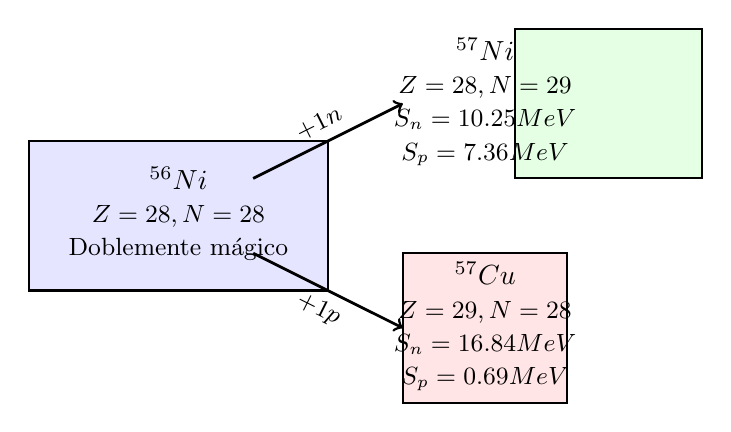
\begin{tikzpicture}[scale=0.95]
  % Carozo 56Ni
  \draw[thick, fill=blue!10] (-5,-1) rectangle (-1,1);
  \node at (-3,0) {\begin{tabular}{c}\textbf{${}^{56}\text{Ni}$}\\ \small $Z=28, N=28$\\ \small Doblemente mágico\end{tabular}};
  
  % 57Ni
  \draw[thick, fill=green!10] (1.5,0.5) rectangle (4,2.5);
  \node at (1.1,1.5) {\begin{tabular}{c}\textbf{${}^{57}\text{Ni}$}\\ \small $Z=28, N=29$\\ \small $S_n = 10.25\text{ MeV}$\\ \small $S_p = 7.36\text{ MeV}$\end{tabular}};
  
  % 57Cu
  \draw[thick, fill=red!10] (0,-2.5) rectangle (2.2,-0.5);
  \node at (1.1,-1.5) {\begin{tabular}{c}\textbf{${}^{57}\text{Cu}$}\\ \small $Z=29, N=28$\\ \small $S_n = 16.84\text{ MeV}$\\ \small $S_p = 0.69\text{ MeV}$\end{tabular}};

  % Flechas
  \draw[->, line width=1pt] (-2,0.5) -- (0,1.5) node[midway, above, sloped] {\small $+1n$};
  \draw[->, line width=1pt] (-2,-0.5) -- (0,-1.5) node[midway, below, sloped] {\small $+1p$};
\end{tikzpicture}
\end{center}

\end{problema}

\newpage

\begin{problema}[Fórmula Semiempírica de la Masa y Estabilidad Nuclear del ${}^{235}\text{U}$ y ${}^{138}\text{Xe}$]
A partir de la expresión para la energía de ligadura nuclear $B(Z,A)$ empleada en la fórmula semiempírica de la masa (SEMF) de Weizsäcker:
\begin{equation}
B(Z,A) = a_V A - a_S A^{2/3} - a_C Z(Z-1) A^{-1/3} - a_A \frac{(A-2Z)^2}{A} + \delta(Z,A)
\end{equation}
donde el término de apareamiento es:
\begin{equation}
\delta(Z,A) = 
\begin{cases} 
+a_P A^{-1/2}, & \text{núcleos par-par} \\ 
0, & \text{núcleos par-impar / impar-par} \\ 
-a_P A^{-1/2}, & \text{núcleos impar-impar} 
\end{cases}
\end{equation}

Se pide:
\begin{enumerate}[label=\alph*)]
    \item Determinar la expresión analítica del número atómico $Z_{\text{est}}$ del núcleo más estable para un número másico $A$ dado.
    \item Estudiar la estabilidad del ${}^{235}\text{U}$ frente a la emisión de un protón, un neutrón y una partícula $\alpha$. Calcular la energía cinética de las partículas $\alpha$ emitidas espontáneamente y comparar el resultado con el valor experimental.
    \item Calcular el valor del número másico $A$ a partir del cual el proceso de desintegración $\alpha$ resulta energéticamente favorable ($Q_\alpha > 0$).
    \item Averiguar si el nucleido radiactivo ${}^{138}\text{Xe}$ es un emisor $\beta^-$ o $\beta^+$.
\end{enumerate}

\textbf{Datos:} $a_V = 15.8\text{ MeV}$, $a_S = 18.3\text{ MeV}$, $a_C = 0.7\text{ MeV}$, $a_A = 23.2\text{ MeV}$, $a_P = 11.2\text{ MeV}$, $m_p = 1.0073\text{ u}$, $m_n = 1.0087\text{ u}$, $m_\alpha = 4.0015\text{ u}$ y $1\text{ u} \cdot c^2 = 931.5\text{ MeV}$.

\tcblower

\subsubsection*{a) Número atómico del isóbaro más estable ($Z_{\text{est}}$)}

La masa atómica $M(Z,A)$ de un núclido neutro expresada en unidades de energía es:
\begin{equation}
M(Z,A) c^2 = Z m_p c^2 + (A-Z) m_n c^2 - B(Z,A)
\end{equation}

Para un número másico $A$ constante, la condición de estabilidad frente a la desintegración $\beta$ se obtiene minimizando la masa respecto a $Z$, considerando el término de apareamiento $\delta$ constante de forma promediada:
\begin{equation}
\frac{\partial (M c^2)}{\partial Z} = (m_p - m_n)c^2 - \frac{\partial B}{\partial Z} = 0
\end{equation}

Derivando la energía de ligadura $B(Z,A)$ respecto a $Z$:
\begin{equation}
\frac{\partial B}{\partial Z} = -a_C (2Z - 1) A^{-1/3} + \frac{4 a_A (A - 2Z)}{A} = -2 a_C Z A^{-1/3} + a_C A^{-1/3} + 4 a_A - \frac{8 a_A Z}{A}
\end{equation}

Igualando las derivadas:
\begin{equation}
(m_p - m_n)c^2 + 2 a_C Z A^{-1/3} - a_C A^{-1/3} - 4 a_A + \frac{8 a_A Z}{A} = 0
\end{equation}

Agrupando los términos proporcionales a $Z$:
\begin{equation}
Z \left[ 2 a_C A^{-1/3} + \frac{8 a_A}{A} \right] = (m_n - m_p)c^2 + 4 a_A + a_C A^{-1/3}
\end{equation}

Despejando $Z_{\text{est}}$ dividiendo numerador y denominador entre $8 a_A / A$:
\begin{equation}
Z_{\text{est}} = \frac{A}{2 + \frac{a_C}{2 a_A} A^{2/3}} \cdot \left[ 1 + \frac{(m_n - m_p)c^2 + a_C A^{-1/3}}{4 a_A} \right] \approx \frac{A}{2 + \left(\frac{a_C}{2 a_A}\right) A^{2/3}}
\end{equation}

Sustituyendo los coeficientes $a_C = 0.7\text{ MeV}$ y $a_A = 23.2\text{ MeV}$:
\begin{equation}
Z_{\text{est}} \approx \frac{A}{2 + 0.0151 \, A^{2/3}}
\end{equation}

\subsubsection*{b) Estabilidad del ${}^{235}\text{U}$ frente a la emisión de $p$, $n$ y $\alpha$}

Calculamos en primer lugar las energías de ligadura $B(Z,A)$ de los núcleos involucrados utilizando la SEMF:

\begin{center}
\begin{tabular}{cccccc}
\hline
Núcleo & $Z$ & $A$ & Tipo & $\delta\text{ (MeV)}$ & $B(Z,A)\text{ (MeV)}$ \\
\hline
${}^{235}\text{U}$ & 92 & 235 & Par-Impar & $0.00$ & $1809.67$ \\
${}^{234}\text{Pa}$ & 91 & 234 & Impar-Impar & $-11.2 \times 234^{-1/2} = -0.73$ & $1803.86$ \\
${}^{234}\text{U}$ & 92 & 234 & Par-Par & $+11.2 \times 234^{-1/2} = +0.73$ & $1804.14$ \\
${}^{231}\text{Th}$ & 90 & 231 & Par-Impar & $0.00$ & $1785.80$ \\
\hline
\end{tabular}
\end{center}

Para la partícula $\alpha$ (${}^4\text{He}$), evaluamos su energía de ligadura a partir de sus masas constituyentes:
\[
\begin{array}{rl}
    B(\alpha) & \displaystyle = \left[ 2 m_p + 2 m_n - m_\alpha \right] c^2 = \\[4pt]
    & \displaystyle = \left[ 2(1.0073) + 2(1.0087) - 4.0015 \right] \times 931.5\text{ MeV} = 28.41\text{ MeV}
\end{array}
\]
Evaluamos la viabilidad energética a través de los valores $Q$:

\paragraph{1. Emisión de protón (${}^{235}\text{U} \to {}^{234}\text{Pa} + p$):}
\begin{equation}
Q_p = B({}^{234}\text{Pa}) - B({}^{235}\text{U}) = 1803.86\text{ MeV} - 1809.67\text{ MeV} = -5.81\text{ MeV} < 0
\end{equation}
Al ser $Q_p < 0$, el ${}^{235}\text{U}$ es \textbf{estable} frente a la emisión de un protón.

\paragraph{2. Emisión de neutrón (${}^{235}\text{U} \to {}^{234}\text{U} + n$):}
\begin{equation}
Q_n = B({}^{234}\text{U}) - B({}^{235}\text{U}) = 1804.14\text{ MeV} - 1809.67\text{ MeV} = -5.53\text{ MeV} < 0
\end{equation}
Al ser $Q_n < 0$, el ${}^{235}\text{U}$ es \textbf{estable} frente a la emisión de un neutrón.

\paragraph{3. Emisión de partícula $\alpha$ (${}^{235}\text{U} \to {}^{231}\text{Th} + \alpha$):}

\[
\begin{array}{rl}
    Q_\alpha & \displaystyle = B({}^{231}\text{Th}) + B(\alpha) - B({}^{235}\text{U}) = \\[4pt]
    & \displaystyle = 1785.80\text{ MeV} + 28.41\text{ MeV} - 1809.67\text{ MeV} = +4.54\text{ MeV} > 0
\end{array}
\]

Como $Q_\alpha > 0$, la desintegración $\alpha$ es \textbf{espontáneamente favorable}.

Por conservación del momento en un sistema de dos cuerpos en reposo, la energía cinética $T_\alpha$ se obtiene mediante el retroceso del núcleo hijo:
\begin{equation}
T_\alpha = Q_\alpha \cdot \left( \frac{A - 4}{A} \right) = 4.54\text{ MeV} \times \left( \frac{231}{235} \right) \approx 4.46\text{ MeV}
\end{equation}

\textit{Comparación experimental:} El valor medido experimentalmente para el ${}^{235}\text{U}$ es $T_\alpha \approx 4.40\text{ MeV}$ ($Q_\alpha \approx 4.68\text{ MeV}$), lo que refleja una excelente precisión del modelo semiempírico.

\subsubsection*{c) Número másico límite para la desintegración $\alpha$ ($Q_\alpha > 0$)}

El valor $Q$ para la emisión de una partícula $\alpha$ se aproxima diferencialmente como:
\begin{equation}
Q_\alpha = B(Z-2, A-4) + B(\alpha) - B(Z,A) \approx B(\alpha) - 4 \frac{\partial B}{\partial A} - 2 \frac{\partial B}{\partial Z}
\end{equation}

Para núcleos situados a lo largo de la línea de estabilidad ($Z \approx Z_{\text{est}}$), se cumple $\frac{\partial B}{\partial Z} \approx (m_n - m_p)c^2 \approx 1.30\text{ MeV}$. Por tanto, la condición de emisión espontánea $Q_\alpha > 0$ exige:
\begin{equation}
4 \frac{\partial B}{\partial A} < B(\alpha) - 2(1.30\text{ MeV}) = 28.41\text{ MeV} - 2.60\text{ MeV} = 25.81\text{ MeV} \implies \frac{\partial B}{\partial A} < 6.45\text{ MeV}
\end{equation}

A medida que $A$ aumenta, la repulsión de Coulomb diminuye drásticamente la ligadura marginal $\frac{\partial B}{\partial A}$. Evaluando las derivadas de la SEMF para $Z \approx 0.4 A$, la desigualdad se satisface a partir de:
\begin{equation}
A \gtrsim 140 - 150
\end{equation}
Esto explica por qué los emisores $\alpha$ espontáneos aparecen en la naturaleza únicamente para $A > 140$.

\subsubsection*{d) Tipo de emisión para el ${}^{138}\text{Xe}$}

Para $A = 138$, calculamos el número atómico del isóbaro estable mediante la expresión obtenida en el apartado a):
\begin{equation}
Z_{\text{est}} \approx \frac{138}{2 + 0.0151 \times (138)^{2/3}} = \frac{138}{2 + 0.0151 \times 26.70} = \frac{138}{2.403} \approx 57.4 \implies Z_{\text{est}} \approx 57 \quad ({}^{138}\text{La})
\end{equation}

El nucleido ${}^{138}\text{Xe}$ posee $Z = 54$ y $N = 138 - 54 = 84$. Al tener $Z = 54 < Z_{\text{est}}$, el ${}^{138}\text{Xe}$ se halla a la izquierda de la parábola de estabilidad, presentando un \textbf{exceso de neutrones}.

Para aproximarse al mínimo de masa $Z_{\text{est}} \approx 57$, debe aumentar su carga atómica $Z$ mediante la transformación débiles de un neutrón en un protón:
\begin{equation}
n \longrightarrow p + e^- + \bar{\nu}_e
\end{equation}

Por lo tanto, el ${}^{138}\text{Xe}$ es un \textbf{emisor $\beta^-$}.

\subsubsection*{Esquema de las Vías de Decaimiento del ${}^{235}\text{U}$}

\begin{center}
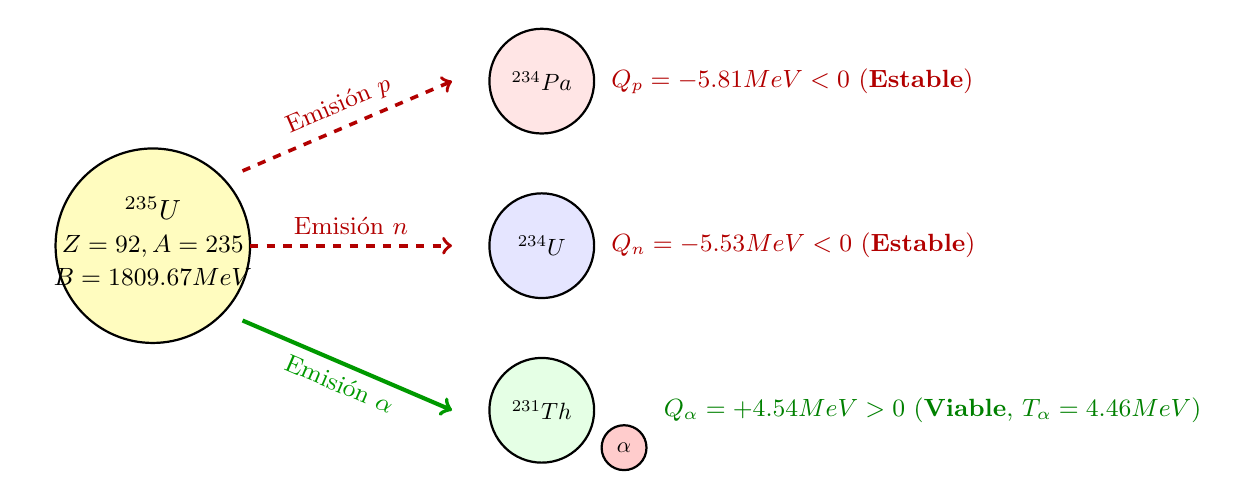
\begin{tikzpicture}[scale=0.95]
  % Núcleo Padre 235U
  \draw[thick, fill=yellow!25] (0,0) circle (1.3) node[black] {\begin{tabular}{c}\textbf{${}^{235}\text{U}$}\\ \small $Z=92, A=235$\\ \small $B = 1809.67\text{ MeV}$\end{tabular}};

  % Emisión p (Prohibida)
  \draw[->, line width=1.3pt, red!70!black, dashed] (1.2,1.0) -- (4.0,2.2) node[midway, above, sloped] {\small Emisión $p$};
  \draw[thick, fill=red!10] (5.2,2.2) circle (0.7) node[black, scale=0.85] {${}^{234}\text{Pa}$};
  \node[red!70!black, right] at (6.0,2.2) {\small $Q_p = -5.81\text{ MeV} < 0$ (\textbf{Estable})};

  % Emisión n (Prohibida)
  \draw[->, line width=1.3pt, red!70!black, dashed] (1.3,0) -- (4.0,0) node[midway, above] {\small Emisión $n$};
  \draw[thick, fill=blue!10] (5.2,0) circle (0.7) node[black, scale=0.85] {${}^{234}\text{U}$};
  \node[red!70!black, right] at (6.0,0) {\small $Q_n = -5.53\text{ MeV} < 0$ (\textbf{Estable})};

  % Emisión alpha (Permitida)
  \draw[->, line width=1.5pt, green!60!black] (1.2,-1.0) -- (4.0,-2.2) node[midway, below, sloped] {\small Emisión $\alpha$};
  \draw[thick, fill=green!10] (5.2,-2.2) circle (0.7) node[black, scale=0.85] {${}^{231}\text{Th}$};
  \draw[thick, fill=red!20] (6.3,-2.7) circle (0.3) node[black, scale=0.8] {$\alpha$};
  \node[green!50!black, right] at (6.7,-2.2) {\small $Q_\alpha = +4.54\text{ MeV} > 0$ (\textbf{Viable}, $T_\alpha = 4.46\text{ MeV}$)};
\end{tikzpicture}
\end{center}

\end{problema}